% =====================================================================
%  Além dos quilômetros: conectividade da rede cicloviária de Fortaleza
%  Trabalho final — artigo de no máximo 3 páginas com elemento gráfico
%
%  Compilar com: powershell -File texto/compilar.ps1
%  (pdflatex -> bibtex -> pdflatex 2x)
% =====================================================================
\documentclass[10pt,a4paper,twocolumn]{article}

\usepackage[utf8]{inputenc}
\usepackage[T1]{fontenc}
\usepackage[brazilian]{babel}
\usepackage[top=2cm,bottom=2cm,left=1.8cm,right=1.8cm,columnsep=0.65cm]{geometry}
\usepackage{graphicx}
\usepackage{caption}
\usepackage{xcolor}
\usepackage{lmodern}
\usepackage{microtype}
\usepackage{flushend}
\usepackage{titlesec}
\usepackage{icomma}
\usepackage[colorlinks=true,allcolors=blue!70!black]{hyperref}

\graphicspath{{../figuras/}{figuras/}} % ../figuras/ localmente; figuras/ no Overleaf
\captionsetup{font=small,labelfont=bf}

% Espaçamentos compactos para seções e parágrafos
\titleformat{\section}{\large\bfseries}{\thesection}{0.7em}{}
\titlespacing*{\section}{0pt}{1.3ex plus .3ex minus .2ex}{0.7ex plus .2ex}
\newcommand{\rotuloparagrafo}[1]{#1.}
\titleformat{\paragraph}[runin]{\normalfont\bfseries}{\theparagraph}{0em}{\rotuloparagrafo}
\titlespacing*{\paragraph}{0pt}{0.7ex plus .2ex minus .1ex}{0.55em}

\pagestyle{empty}
\renewcommand{\topfraction}{0.88}
\renewcommand{\floatpagefraction}{0.75}

\begin{document}

% ---------------------------------------------------------------- cabeçalho e título
\twocolumn[
\begin{@twocolumnfalse}
\begin{center}
\IfFileExists{figs/unifor_logo.png}
  {
\includegraphics[height=1.4cm]{figs/unifor_logo.png}\par\vspace{0.2cm}}
  {\fbox{\parbox{5.5cm}{\centering\footnotesize\color{red}[inserir \texttt{texto/figs/unifor\_logo.png}]}}\par\vspace{0.2cm}}

{\footnotesize\bfseries Universidade de Fortaleza (UNIFOR) \quad$\cdot$\quad Centro de Ciências Tecnológicas\\
Programa de Pós-Graduação em Informática Aplicada (PPGIA)\\
Ciência de Dados Aplicada à Ciência da Cidade \quad$\cdot$\quad novembro de 2026\par}

\vspace{0.35cm}
{\LARGE\bfseries Além dos quilômetros\par}
\vspace{0.18cm}
{\large Conectividade da rede cicloviária de Fortaleza\par}
\vspace{0.25cm}
{\normalsize\textbf{Sara Pessoa}\par}
{\footnotesize Mestrado em Informática Aplicada\par}
\vspace{0.35cm}
\end{center}

\begin{quote}\small
\noindent\textbf{Resumo.}
A extensão da malha cicloviária é o indicador mais divulgado, mas não informa se os trechos estão ligados entre si nem a quem servem. Neste trabalho, as ciclovias e ciclofaixas de Fortaleza, obtidas de dados públicos, são representadas como um grafo e cruzadas com os setores do Censo 2022. Os 429~km analisados formam 44 componentes. O maior reúne 56\% da extensão, e dois conjuntos, a oeste e a sudeste, somam 131~km sem ligação com ele; cerca de 1,4~km de ligações pelas ruas reuniria 90\% da rede. A fragmentação tem recorte de renda. A até 300~m pelas ruas, 66\% dos moradores do décimo mais rico estão perto do maior componente, contra 11\% no mais pobre, e a desigualdade no acesso à parte conectada é o dobro da desigualdade na simples cobertura. A ligação do conjunto oeste, marcada no OpenStreetMap em 2024 mas ausente da base oficial, reduz essa desigualdade à metade.

\vspace{0.15cm}
\noindent\textbf{Palavras-chave:} redes espaciais, componentes conectados, infraestrutura cicloviária, Fortaleza.
\end{quote}
\vspace{0.35cm}
\end{@twocolumnfalse}
]

% ---------------------------------------------------------------- problema
\section{Qual é o problema?}

Fortaleza ampliou sua infraestrutura cicloviária na última década, orientada
pelo Plano Diretor Cicloviário Integrado, que prevê 524~km até 2030. O avanço
dessa política costuma ser divulgado como a fração dessa meta de extensão já
implantada~\cite{opovo2022}. Para quem pedala, porém, importa também se os
trechos se ligam: uma ciclofaixa isolada pouco amplia os destinos alcançáveis
com segurança. Hansen~\cite{hansen1959} definiu acessibilidade como o potencial
de oportunidades de interação, ponderado pela separação espacial entre elas.
Trechos isolados reduzem as oportunidades alcançáveis pela infraestrutura
dedicada. Estudos recentes sobre cidades de 15 minutos e sobre o acesso a
serviços por bicicleta ou a pé reforçam essa leitura~\cite{bruno2024,xu2020}.

Na ciência das cidades, infraestruturas urbanas são tratadas como redes
espaciais~\cite{bettencourt2021,maia2023}. Para redes cicloviárias, Natera
Orozco \emph{et al.}~\cite{natera2020} mostraram que mesmo cidades com
tradição de uso da bicicleta têm redes formadas por centenas de fragmentos
desconectados. Szell \emph{et al.}~\cite{szell2022} encontraram retornos
decrescentes do investimento até que a rede ultrapasse um limiar crítico, a
partir do qual a conectividade cresce. A revisão de Buehler e
Dill~\cite{buehler2016} aponta que medidas de rede, e não apenas de extensão,
ainda são pouco usadas para avaliar infraestrutura cicloviária. Bruno
\emph{et al.}~\cite{bruno2024} mostram que o acesso por proximidade se distribui
de forma desigual dentro das cidades, o que pede olhar também para quem a rede
alcança.

Este trabalho investiga a seguinte questão: \textbf{as ciclovias e ciclofaixas
de Fortaleza formam uma rede contínua ou conjuntos de trechos desconectados
entre si, e quem fica perto da parte conectada?}

% ---- figura
\begin{figure*}[t]
\centering
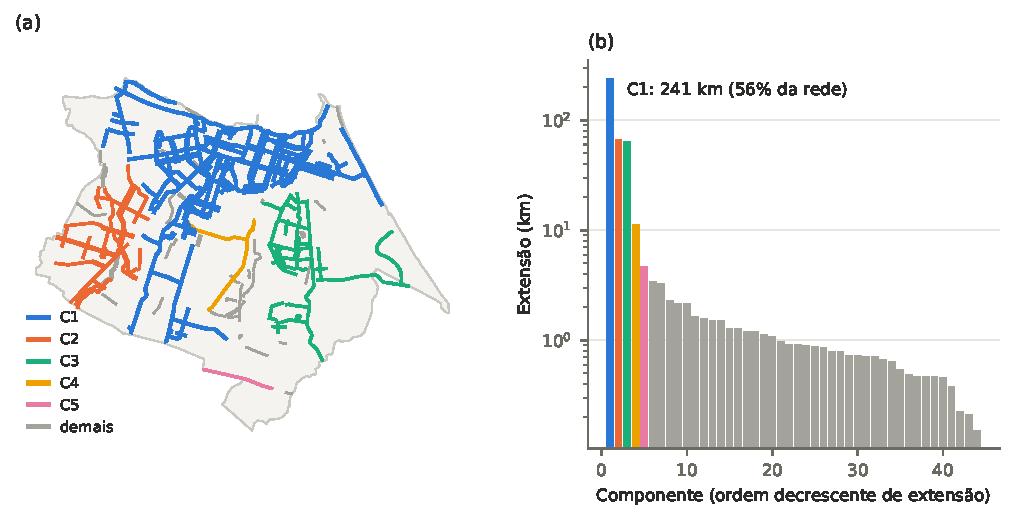
\includegraphics[width=\textwidth]{conectividade.pdf}
\caption{\textbf{Componentes conectados da rede cicloviária de Fortaleza.} \textbf{(a)} Ciclovias e ciclofaixas coloridas pelos cinco maiores componentes conectados (tolerância de 10~m, sem as passagens em desnível). Os círculos marcam a ligação C1--C2 registrada no OpenStreetMap em 2024, ausente da base, e a menor ligação pelas ruas entre C1 e C3. \textbf{(b)} Moradores a até 300~m pelas ruas de algum trecho, de C1 e de C1 ou C2, por décimo de renda do setor censitário; entre parênteses, o índice de concentração. \textbf{(c)} Fração da rede no maior componente à medida que se acrescentam ligações pelas ruas, em duas ordens de escolha.}
\label{fig:conectividade}
\end{figure*}

% ---------------------------------------------------------------- método
\section{O que foi feito}

\paragraph{Dados} Utilizou-se a malha cicloviária publicada pela Prefeitura
no portal de dados abertos~\cite{fortaleza2024}. O arquivo foi atualizado no
catálogo em junho de 2024, mas a maioria dos trechos tem 2022 como ano de
referência. Foram mantidos os 406 trechos de ciclovias (139,6~km) e
ciclofaixas (289,7~km), que somam 429,3~km; ciclorrotas e passeios
compartilhados (17~km) foram excluídos por não oferecerem espaço exclusivo à
bicicleta. Os moradores e o rendimento médio dos responsáveis pelos domicílios
vêm dos 4\,408 setores censitários de Fortaleza no Censo 2022~\cite{ibge2022}.
As distâncias foram medidas em metros, em SIRGAS~2000/UTM~24S.

\paragraph{Construção da rede} Construiu-se um grafo não direcionado em que
dois trechos são adjacentes quando se cruzam ou quando a extremidade de um
está a até 10~m de qualquer ponto do outro. A tolerância absorve imprecisões
de desenho, e a análise foi repetida com tolerâncias de 0 a 50~m. Adotou-se
10~m porque, a partir desse valor, o maior componente fica praticamente
estável (56,1\% a 56,5\% da extensão até 50~m). O indicador principal é a
fração da extensão contida no maior componente.

\paragraph{Conferência das conexões} Como proximidade no mapa não garante
passagem, 77 das 275 conexões incertas foram conferidas em imagem de satélite:
as 39 críticas, cuja remoção separaria partes da rede, as 18 junto a pontes,
viadutos ou túneis no OpenStreetMap~\cite{osm2026} e 20 sorteadas. As 11
passagens em desnível encontradas foram removidas.

\paragraph{Ligações faltantes} Para os componentes seguintes ao maior, mediu-se
a menor ligação até ele pela malha viária do OpenStreetMap e verificou-se se a
infraestrutura cicloviária registrada hoje no OpenStreetMap já a faz. Para
estimar quanta infraestrutura uniria a rede, adaptou-se a estratégia gulosa de
Natera Orozco \emph{et al.}~\cite{natera2020}: a cada passo, o maior componente
é ligado a outro pelo menor caminho nas ruas, que passa a integrá-lo.
Compararam-se duas regras: o componente mais próximo e o que acrescenta mais
extensão por metro de ligação.

\paragraph{População atendida} A população de cada setor foi repartida numa
grade de 50~m, supondo-a uniforme na área do setor. Um morador é considerado
perto de um componente se algum trecho dele estiver a até 300~m pelas ruas do
OpenStreetMap. A desigualdade foi medida por décimos de renda dos setores,
ponderados pela população, e pelo índice de concentração~\cite{wagstaff1991}:
vale 0 quando o acesso se distribui por igual entre ricos e pobres e é positivo
quando se concentra nos de maior renda. O código e os dados estão em
\url{https://github.com/Sarapessoa/artigo-ciencia-cidades}.

% ---------------------------------------------------------------- resultados
\section{Resultados e conclusões}

A rede analisada forma 44 componentes, dos quais 32 são trechos isolados
(Fig.~\ref{fig:conectividade}a). O maior componente (C1) tem 241~km, ou 56\% da
extensão total, e cobre o Centro, a orla e um eixo que segue do centro para o
sul. Seguem dois componentes regionais. C2 (67~km), a oeste, inclui Antônio
Bezerra, Bom Jardim e Conjunto Ceará. C3 (64~km), a sudeste, inclui Cambeba,
Cidade dos Funcionários e Edson Queiroz. Os demais 41 têm menos de 12~km cada.

Em linha reta, C2 e C3 estão a 344~m e 686~m de C1, mas essas distâncias
enganam: a de C2 cai sob o Viaduto Antônio Bezerra, e a de C3 atravessa a mata
do Parque do Cocó. A conferência com o OpenStreetMap mudou a leitura de C2: uma
ciclofaixa de 0,8~km no viaduto e nas ruas vizinhas, marcada em 2024 e visível
em imagem de satélite, já liga C2 a C1, mas não consta da base. Com ela, o
maior componente reuniria 72\% da extensão. C3 continua separado nas duas
fontes; a menor ligação pelas ruas tem 799~m, cruzando o Rio Cocó pela
Av.~Eng. Santana Júnior, sem infraestrutura cicloviária.

A curva das ligações faltantes (Fig.~\ref{fig:conectividade}c) generaliza esse
resultado. Escolhendo a cada passo o maior ganho por metro, 1,4~km de ligações,
que unem C4, C2 e C3 ao maior componente, elevam sua fração de 56\% para 90\%.
Ligar sempre o mais próximo exige 5,5~km para o mesmo resultado, e os últimos
5\%, formados por fragmentos isolados, consomem a maior parte dos 18~km
necessários para conectar tudo. É o padrão descrito por Natera Orozco \emph{et
al.}~\cite{natera2020}: poucos trechos curtos e bem posicionados consolidam
redes fragmentadas.

A fragmentação pesa mais sobre os mais pobres (Fig.~\ref{fig:conectividade}b).
A até 300~m pelas ruas, 48\% dos moradores têm algum trecho por perto, mas só
28\% estão perto de C1. No décimo de renda mais pobre, 35\% têm algum trecho
por perto, e só um terço deles está perto de C1; no mais rico, são 78\% e
84\%. O índice de concentração do acesso a C1 (0,33) é o dobro do de ter
algum trecho por perto (0,15): a rede chega aos bairros pobres, mas em pedaços
desconectados. C2 atende sobretudo bairros de baixa renda do oeste, como Bom
Jardim, Bonsucesso e Canindezinho, e sua ligação, já registrada no
OpenStreetMap, reduz o índice para 0,17 e eleva o atendimento do décimo mais
pobre de 11\% para 26\%. Escolhidas pelo ganho em moradores, as ligações
seguem quase a mesma ordem, com C2 primeiro, e 1,6~km atendem 90\% da
população próxima à rede.

Os resultados são robustos. Entre 5 e 50~m de tolerância, o maior componente
reúne de 52\% a 57\% da extensão; das 77 conexões conferidas, 63 eram
encontros em nível, e retirar também as 3 inconclusivas o reduz a 55\%. O
gradiente de renda se mantém a 200 e 500~m, em linha reta e incluindo
calçadas e caminhos de pedestres.

\paragraph{Conclusão} A rede de ciclovias e ciclofaixas de Fortaleza
registrada na base oficial não é contínua: pouco mais da metade da extensão
está em um único componente, e a extensão total superestima a rede utilizável
sem trechos em tráfego misto. Essa fragmentação não é neutra: os moradores de
baixa renda têm infraestrutura por perto com menos frequência e, quando têm,
ela pertence mais vezes a pedaços desconectados. Parte do problema já foi
resolvida depois da base: a ligação de C2, ausente do registro oficial, é a
que mais reduz essa desigualdade. A separação mais relevante que resta é a do
sudeste: somadas à ligação de C2, cerca de 0,9~km de novas ligações, até C3 e
C4, reuniriam 89\% da extensão em um só componente. Para a conectividade, a localização dos novos trechos pesa mais
que sua extensão. Ligar componentes, porém, não resolve a cobertura: metade
dos moradores não tem nenhum trecho a até 300~m, sobretudo nas bordas sul da
cidade, como Jangurussu e Mondubim.

\paragraph{Limitações} Uma desconexão na base não impede a circulação de
bicicleta pelas vias comuns; indica apenas a falta de infraestrutura dedicada.
Um encontro em nível não garante travessia sinalizada. O OpenStreetMap é
mantido por voluntários: a ligação de C2 foi confirmada pelo histórico de
edições e por imagem, mas não em campo, e o acesso pelas ruas depende do quanto
as vielas estão mapeadas. As ligações indicam o comprimento mínimo, não a
viabilidade de implantação, e a estratégia gulosa não garante a combinação
ótima. A renda é a média do setor, e a análise não descreve indivíduos. O grafo
não direcionado ignora o sentido de circulação, e a análise não mede
segurança, conservação nem uso.

% ---------------------------------------------------------------- refs
\bibliographystyle{unsrt-pt}
\bibliography{referencias}

\end{document}
